\documentclass[]{standalone} 
\usepackage{pgfplots} 
%\usepgfplotslibrary{external} 
%\tikzexternalize 
\usepgfplotslibrary{fillbetween}
\usetikzlibrary{arrows, decorations.markings}
\usepackage{tikz} 
\usepackage{amsmath} 
\usepackage{pgfplots} 
\usepackage{sansmath}
\sansmath  
\usetikzlibrary{calc} 
\pgfplotsset{compat = newest, every axis plot post/.style={line join=round}, label style={font=\Large},every tick label/.append style={font=\large}  }
\begin{document} 
	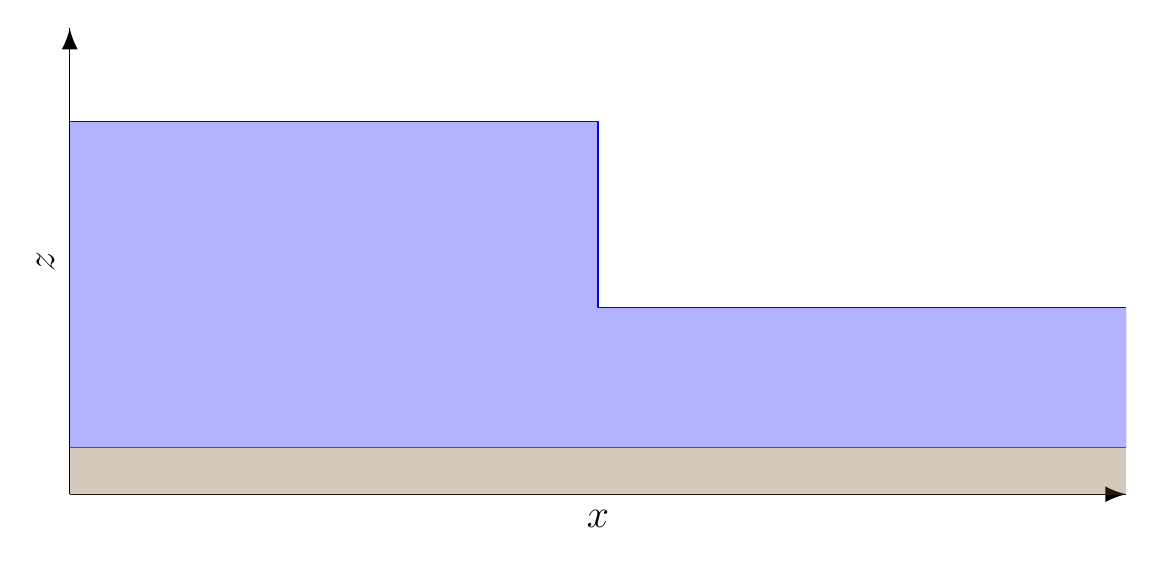
\begin{tikzpicture}
		\makeatletter
		\tikzset{
			nomorepostaction/.code=\makeatletter\let\tikz@postactions\pgfutil@empty, % From https://tex.stackexchange.com/questions/3184/applying-a-postaction-to-every-path-in-tikz/5354#5354
			my axis/.style={
				postaction={
					decoration={
						markings,
						mark=at position 1 with {
							\arrow[ultra thick]{latex}
						}
					},
					decorate,
					nomorepostaction
				},
				thin,
				-, % switch off other arrow tips
				every path/.append style=my axis % this is necessary so it works both with "axis lines=left" and "axis lines=middle"
			}
		}
		\makeatother
	
	\begin{axis}[ 
	width = 0.7\textwidth,
	width=15cm,
	height = 7.5cm,
	axis lines = left, 
	axis line style={my axis},
	xtick={\empty},  
	ytick = {\empty}, 
	xmin=0, 
	xmax=1, 
	ymin =0, 
	ymax = 1,
	xlabel=$x$, 
	ylabel=$z$]
	
	\addplot [name path=b,brown!60!black] coordinates {(0,0.1)  (1,0.1)};
	
	\path[name path=axis] (axis cs:0,-0.05) --  (axis cs:1,-0.05);
	
	\addplot [name path=a,blue] coordinates {(0,0.8) (0.5,0.8) (0.5,0.4) (1,0.4)};
	
		\addplot [
		thick,
		color=brown!60!black,
		fill=brown!60!black, 
		fill opacity=0.3
		] fill between[of=b and axis];
		
	\addplot [
	thick,
	color=blue,
	fill=blue, 
	fill opacity=0.3
	] fill between[of=a and b];
	

	\end{axis} 
	
	
	
	\end{tikzpicture}
\end{document}